\testCom
{%Номер задачи
	3.147
}
{%Условие
	условие
}
{%Дано
	дано
}
{%Найти
	найти
}
{%Решение
	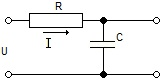
\includegraphics[height=30mm]{3_147.jpg}\\
	$U_0 = 1 + \cos \omega t$\\
	а) Заметим, что $U' = \frac{q}{C}$ и запишем правило Киргофа:\\
	$ I R + I X_C = \tilde U \Rightarrow I = \frac{\tilde U}{R + X_c}, $где $\tilde U = e^i\omega t$\\
	$X_C = - \frac{i}{\omega C}$ - ёмкостное сопротивление\\
	$\tilde U' = \frac{\tilde U}{\omega C R + 1}(1 - i \omega C R) = A e^{i (\omega t + \alpha)}$\\
	$\alpha = - \arctg \omega C R \quad A = \frac{\abs{\tilde U}}{\omega C R + 1} \abs{1 - i \omega C R} = \frac{\abs{\tilde U}}{\sqrt{ (\omega C R)^2 + L}} = \frac{U_0}{\sqrt{L  + (\omega C R)^2 }}$\\
	Постоянная составляющая $U$($H$ пройдёт до $U'$ без изменений, поэтому\\
	$U'(t) = U_0 + Re \tilde U' = (1 + \frac{1}{\sqrt{1 + (\omega C R)^2}} \cos (\omega t - \arctg \omega C R))$\\
	б) $\frac{1}{\sqrt{1 + (\omega C R)^2}} = \frac{1}{\eta} \quad (\omega C R)^2 = \eta^2 - 1, \, CR = \frac{\sqrt{\eta^2 - 1}}{\omega}$\\
}

